\documentclass[12pt,a4paper]{article}
\usepackage{ctex,graphicx,textcomp,amsmath,amsfonts,subfigure,multirow,ulem,listings}
\usepackage{amssymb,indentfirst,bm,subfigure,hyperref,xcolor,pifont}
\usepackage{geometry}
\setlength{\topmargin}{-0.45in}
\setlength{\evensidemargin}{0in}
\setlength{\oddsidemargin}{0in}
\setlength{\textwidth}{6.5in}
\setlength{\textheight}{9.5in}
\setlength{\headsep}{0.25in}

\author{Chen Ying, Zhu Simo, Liu Guoding, Mao Haining}
\title{\textbf{Report for Final Project : Analysis of Rumor}}
\date{January, 2019}
\usepackage{fancyhdr}
\pagestyle{fancy}
\lhead{\textsl{Report for Final Project: Analysis of Rumor}}
\chead{}
\rhead{\textsl{\thepage}}
\usepackage{enumerate}
\usepackage{enumitem}
\setlist[enumerate,1]{label=$\bullet$,font=\textup,
	leftmargin=7mm,labelsep=1.5mm,topsep=0mm,itemsep=-0.8mm}
\setlist[enumerate,2]{label=(\alph*),font=\textup, 
	leftmargin=7mm,labelsep=1.5mm,topsep=-0.8mm,itemsep=-0.8mm}


\begin{document}
\thispagestyle{plain}
\newcommand{\xiaosi}{\fontsize{12pt}{18pt}\selectfont}
\newcommand{\h}{\begin{tabular}{|c|c|}\hline\end{tabular}}
\newcommand{\rd}{\mathrm{d}}
\newcommand{\dps}[1]{\displaystyle{#1}}
\newcommand{\tabincell}[2]{\begin{tabular}{@{}#1@{}}#2\end{tabular}}
\newcommand{\noindentpar}{\hangafter=1 \setlength{\hangindent}{2em}\noindent}

\lstset{language=python,numbers=left, breaklines=true,
	numberstyle=\footnotesize,keywordstyle=\color{blue!100}\fontspec{Consolas Bold},
	commentstyle=\color{red!30!green!90!blue!100}\fontspec{Consolas Italic},stringstyle=\color{red!30!green!50!blue!82},frame=shadowbox,
	rulesepcolor=\color{red!20!green!20!blue!20},basicstyle=\fontspec{Consolas}\footnotesize,tabsize=4,showstringspaces=false,columns=flexible,xleftmargin=2em,xrightmargin=2em, aboveskip=1em}

\newcommand{\fn}[1]{\normalfont{#1}}
\newcommand{\fc}[1]{\fontspec{Consolas}\small{#1}\fn{}}
\renewcommand{\'}{\fc{'}\fn{}}
\newcommand{\ns}{\normalsize}
\renewcommand{\contentsname}{Contents}
\maketitle
\vspace{20pt}
\rule[-10pt]{15cm}{0.05em}
\vspace{-5pt}
\tableofcontents
\vspace{-5pt}
\rule[-10pt]{15cm}{0.05em}
\clearpage
\section{Introduction}
Text data is around us everywhere, and how to deal with those words, sentences or passages has long been a hot topic for natural language processing fields. With the rapid development and popularization of social media services, rumors are spreading with unprecedented rapidity and have a tremendous impact on human society. Meanwhile, the development of artificial intelligence technologies provides a promising approach for social media platform to automatically detect rumors. 

In daily life, people usually distinguish the authenticity of microblog events based on their common sense or through news websites and public communities, however, the reports of this kind of website media are incomplete and have certain time delay. Therefore, the automatic identification of rumor events can help us better prevent rumors and assist management agencies in rumor intervention and governance.

Under that situation, we hope to set up a model to distinguish those rumors from normal ones with only contents rather than making predictions based on all comments when users forward the message. In the following part, we will explain how the semantic and syntactic information influence the authenticity of a given context, how different representing methods and classification models performs on this classification problem, and, finally, how our primary features can be explanatory for deeper analysis of rumor.

\section{Preliminary Process (Data Reading)}
The documents in the dataset are scores of JSON (JavaScript Object Notation) documents, the information contained in one json document has the construct below:

\begin{figure}[htbp]
	\centering
	\begin{minipage}{0.49\linewidth}
		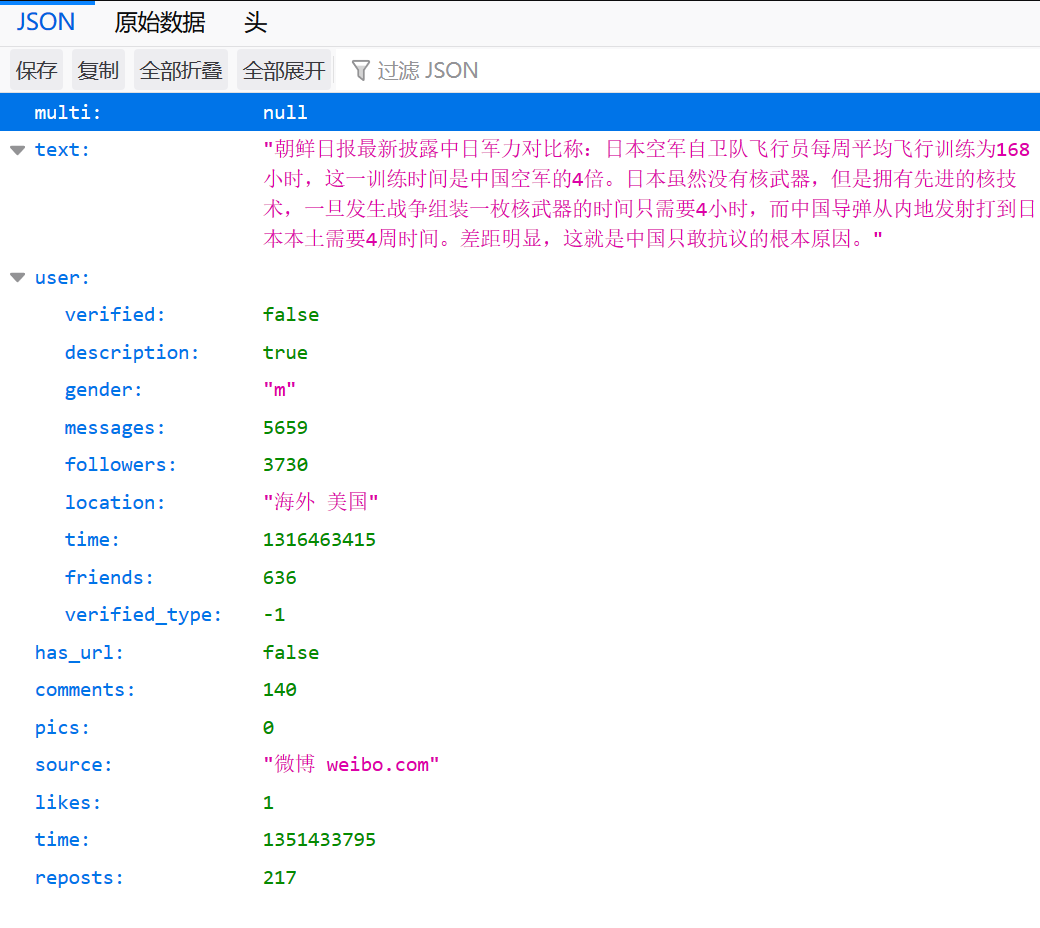
\includegraphics[height=2.8in]{pic/example}
	\end{minipage}
\hfil
	\begin{minipage}{0.49\linewidth}
		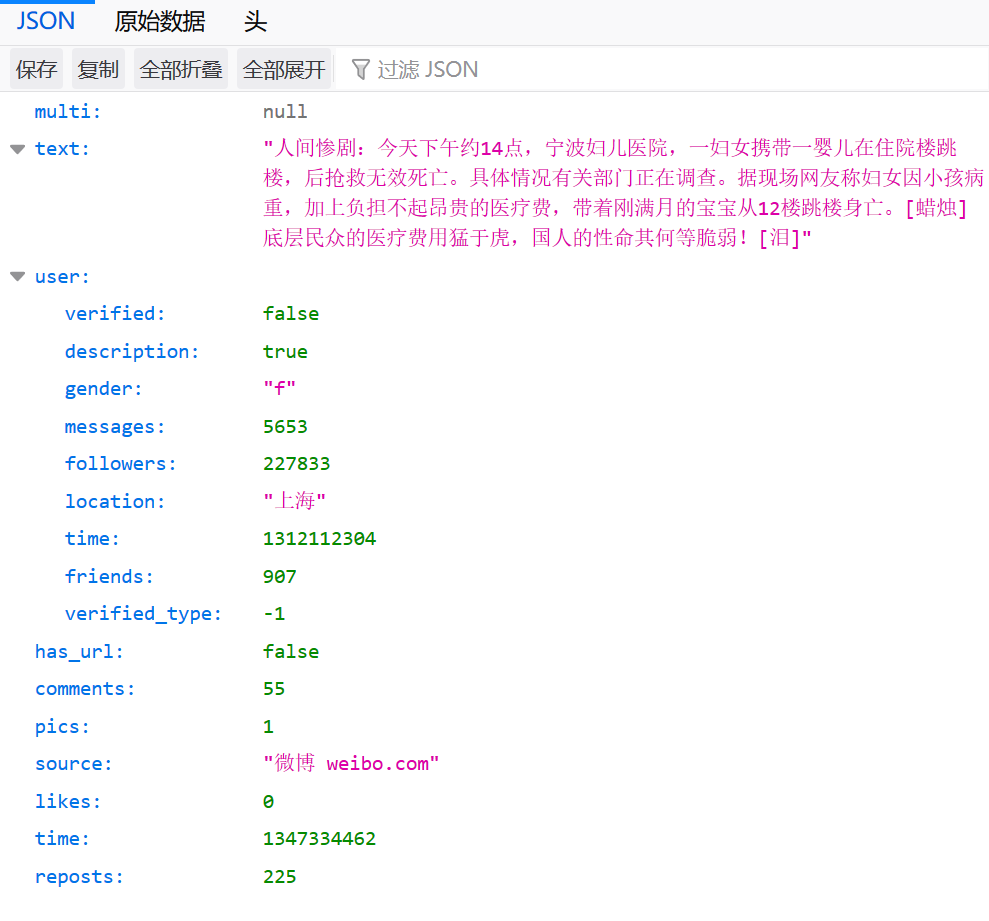
\includegraphics[height=2.8in]{pic/example2}
	\end{minipage}
\end{figure}
\clearpage
The useful information of it contains:

\vspace{1em}
\setlength\parindent{4.5em}
\fbox{\parbox{0.65\linewidth}{
		\begin{enumerate}
		\item Text
		\item Weibo Features
		\begin{enumerate}
			\item Whether the weibo has URL
			\item Number of comments
			\item Pics
			\item Sources of this weibo
			\item Likes
			\item The time when this weibo is sent
		\end{enumerate}
%	\end{enumerate}}}

%\fbox{\parbox{0.65\linewidth}{
%		\begin{enumerate}
		\item User Features
		\begin{enumerate}
			\item Whether the user has description
			\item Whether the user is verified and the verified type
			\item The gender of user
			\item Number of followers
			\item Number of friends
			\item The location of the user
			\item The time when the user joined weibo
			\item Number of messages user had sent
		\end{enumerate}
	\end{enumerate}
}}
\vspace{1em}

\setlength{\parindent}{2em}
To get this information, we preprocess these json documents. In this process, we use the \'\fc{os}\' \& \'\fc{json}\' module to read all the json data and extract information we need. Since the dataset has been processed, there is no missing data (in other words, all the json documents have complete information) or duplicate records, the presentation of features are also consistent, which saves us much effort. 

Then we encode each feature by the method \textbf{ordinary encoding}. First, we use list to collect data, and then transform it into ndarray to adapt (except text data, which will be processed in the feature extraction part). In the meantime, we transform the data type into int (some examples are below).

\begin{lstlisting}
has_url = np.array(has_url).astype(int)
verified = np.array(verified).astype(int)
description = np.array(description).astype(int)
gender = np.array(list(map(trans_gender, gender)))
followers = np.array(followers)
friends = np.array(friends)
category = np.array(category)
\end{lstlisting}
\clearpage
\section{EDA \& Feature Extraction}
In this project, we try to extract features from the information in each json document. Before this project, we read some papers, among which the paper written by Prof. Liu Zhiyuan impressed us most. He asserts that there are several methods to detect rumors according to the features of the time series, but in that method, we can't detect rumors as soon as they are sent. Additionally, stopping the rumor early will help stop the potential social loss. This idea determines the features we finally choose. It should be attached great importance here that in this project we want to extract \textbf{the early characteristics of rumors}. The information of rumor after the time when rumor is sent, such as comments of this rumor isn't considered into this classification model.

First we use Exploratory Data Analysis methods to see the general features of rumors in this dataset and then we select the features which will be used in the model training process. \footnote{In the real process, we must construct feature first and then use EDA to see the characteristics. After this we determine whether we will use these features. The order this report describe is little different from the real order.}
\subsection{Exploratory Data Analysis (EDA)}
In EDA process, we first explore the single feature of rumors as well as non-rumors and then compare them in one picture. For example we count the number of exclamation marks(\textbf{the coordinate has been normalized}) in each text and then describe it through frequency histogram to figure out the characteristic of distribution.

\begin{figure}[htbp]
	\centering
	\begin{minipage}{0.32\linewidth}
		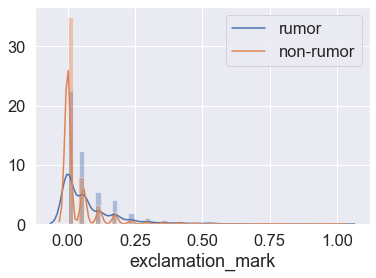
\includegraphics[height=1.8in]{pic/exclamation_mark}
	\end{minipage}
	\hfil
	\begin{minipage}{0.32\linewidth}
		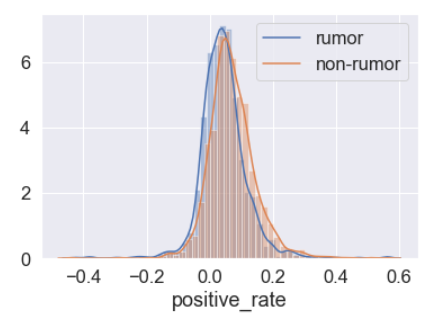
\includegraphics[height=1.8in]{pic/positive_rate}
	\end{minipage}
\end{figure}

\begin{figure}[htbp]
	\centering
	\begin{minipage}{0.32\linewidth}
		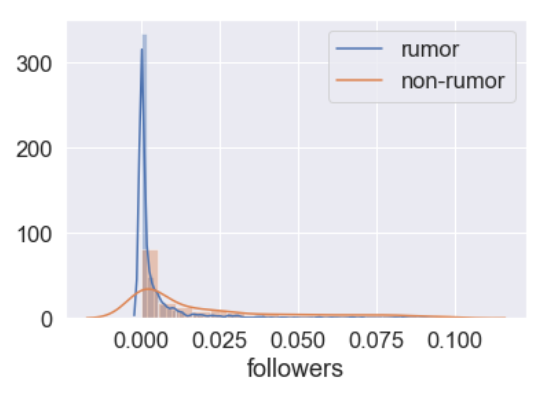
\includegraphics[height=1.8in]{pic/followers}
	\end{minipage}
	\hfil
	\begin{minipage}{0.32\linewidth}
		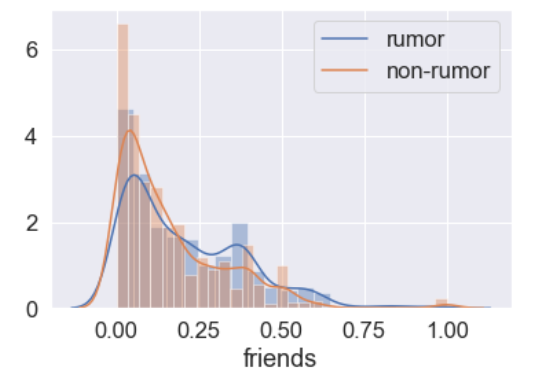
\includegraphics[height=1.8in]{pic/friends}
	\end{minipage}
\end{figure}
\clearpage
In this process, we find that rumors are more frequently expressed with more exclamation marks as well as question marks.\label{2.1marks} Besides, rumors tend to present negative attitude. Meanwhile, we find the number of friends of rumor-mongers' weibo account is statistically larger.

Then we explore \textbf{the correlation between different features} (variables). At the same time, we can see the features more clearly. Actually, none of these features are predominant feature which can almost determine the classification with a relatively high coefficient of association, so the combination of different features may be a good method. 

\begin{figure}[h]
	\centering
	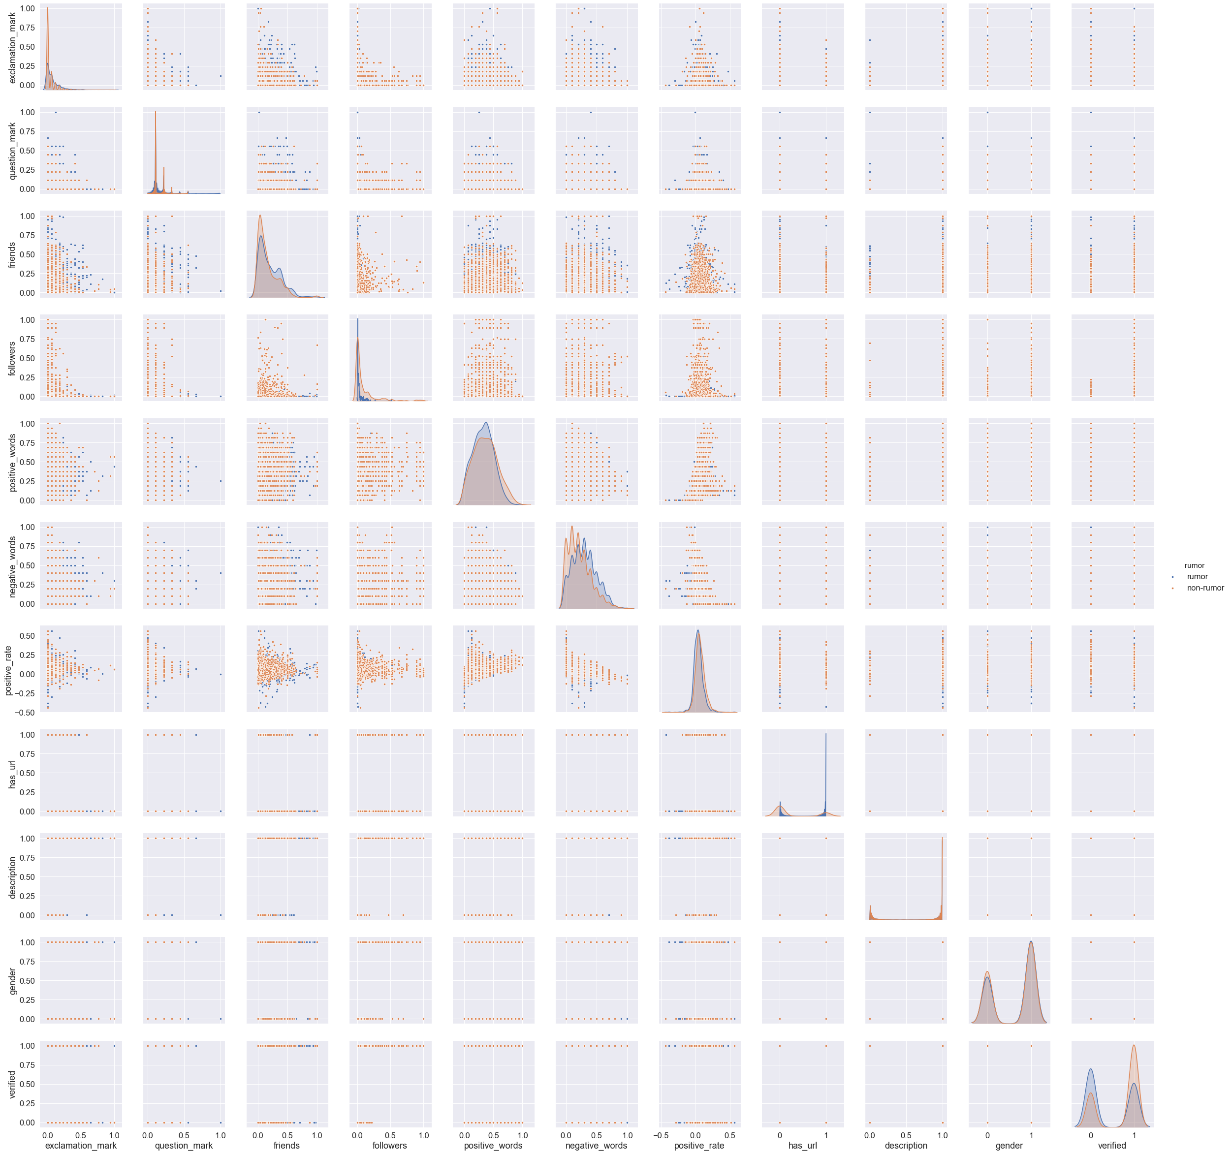
\includegraphics[height=1\linewidth]{pic/pairplot}
\end{figure}

We also find an interesting thing that the positive rate of the rumors is not always low, instead, it is very low or very high. That reminds us the rumors may be too positive or too negative, so decision tree may be a good choice. However, generally speaking, the rumors are always radical.
\clearpage
\begin{figure}[htbp]
	\centering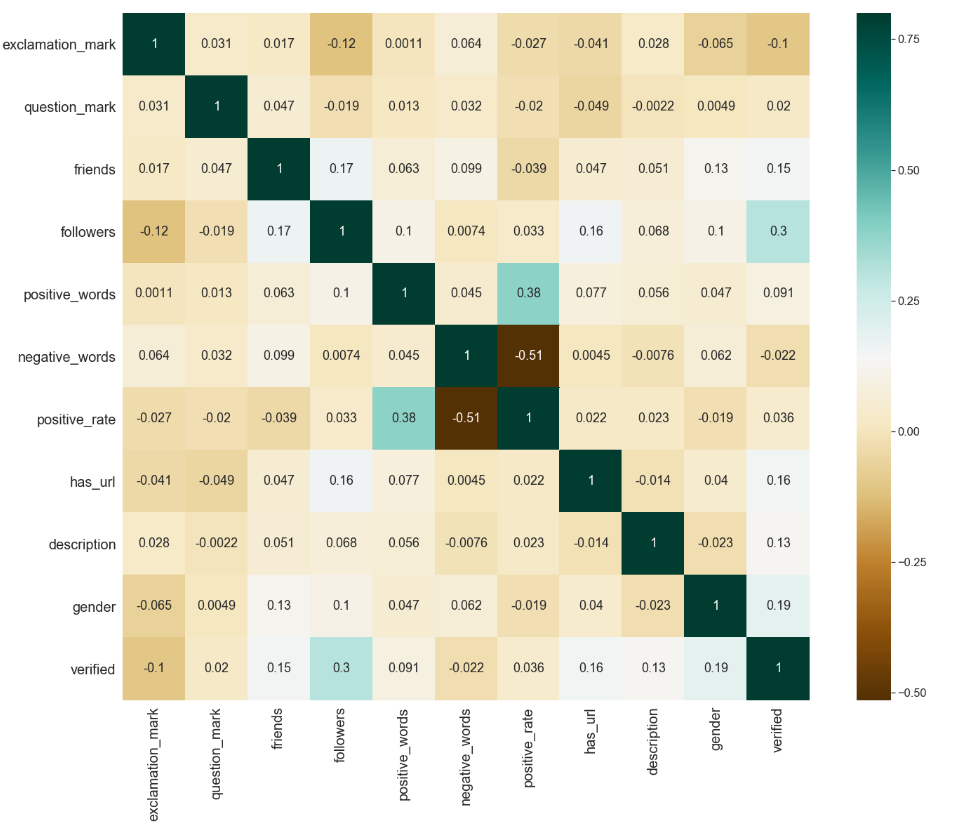
\includegraphics[height=0.86\linewidth]{pic/heatmap}
\end{figure}

\subsection{Feature Extraction}
After the exploration process, considering the construct of the dataset and the characteristics of the rumor texts, we select the features below as the features we aim to extract and use as analytical basis in this classification model.

\vspace{10pt}
\setlength{\parindent}{5em}
\fbox{\parbox{0.65\linewidth}{
\begin{enumerate}
	\item Text Features
	\begin{enumerate}
		\item Number of exclamation marks
		\item Number of question marks
		\item Number of positive words
		\item Number of negative words
		\item Positive rate of the text
	\end{enumerate}
	\item Weibo Features
	\begin{enumerate}
		\item Whether the weibo has URL
	\end{enumerate}
\end{enumerate}}}
\clearpage
\fbox{\parbox{0.65\linewidth}{
		\begin{enumerate}
	\item User Features
	\begin{enumerate}
		\item Whether the user has description
		\item Whether the user is verified
		\item The gender of user
		\item Number of followers
		\item Number of friends
	\end{enumerate}
\end{enumerate}}}
\vspace{10pt}

\setlength{\parindent}{2em}
Since the features (except text features) have been processed in the preliminary process, this time we only need to extract the features from weibo text message mainly through NLP (Natural Language Processing) methods.

This process is hard to handle. We refer to papers in the field of NLP and conclude that \textbf{rumors are always radical}. So we thought about those features which can reflect whether the text is ``radical''. According to the general knowledge of linguistics \sout{(though quite poor)}, finally we select these features to construct our rumor classification model:

\vspace{10pt}
\setlength{\parindent}{5em}
\fbox{\parbox{0.65\linewidth}{
\begin{enumerate}
	\item Number of exclamation marks
	\item 	Number of question marks
	\item 	Number of positive words
	\item 	Number of negative words
	\item 	Positive rate of the text
\end{enumerate}}}
\vspace{10pt}

\setlength{\parindent}{2em}
We use these features for the reason that if one text is radical, it will tend to use more exclamation marks and more question marks\footnote{Just as the explanation we've proposed before in subsection \ref{2.1marks}}. Besides, rumors tend to use more positive or negative words (radical, in summary). In general the tonal of the text will be radical so we try to construct a feature which will reflect this point. 

We know the character of one sentence will be represented by \textbf{the ``key word'' of this sentence}. The ``key word'' in this project is defined:

\begin{quotation}
	The words appeared in this sentence but don't appear in most of sentences we use in daily life.
\end{quotation}

So we want to get the ``key word" and evaluate the text by the ``key word'' of the text. Then we use module jieba to split the raw text message (before this we use regular expression to clean the text) and get the most importance ``key words'' of the text (jieba has a corpus and can return the importance words according to the TF). The number of importance words can be set, which forms a hyper-parameter. 

Once we get the ``key words'', we use SnowNLP module to evaluate the emotion of each word. The value of neutral word is 0.5. The value will be larger if the word is more positive and smaller if the word is more negative. So we count the positive words and negative words of these ``key words'' according to the rule: if the value is larger than 0.6, the word is positive word. If the value is smaller than 0.4, the word is negative word.

\begin{lstlisting}
for x, w in jieba.analyse.textrank(sent, topK=top_word, withWeight=True,allowPOS=allowpos):
	rate += (SnowNLP(x).sentiments - 0.5) * w
	if (SnowNLP(x).sentiments < 0.4):
		negative_num += 1
	if (SnowNLP(x).sentiments > 0.6):
		postive_num += 1
##加上最后一个0.000000001是因为有的微博没有关键词,所以为了防止分母为0加上一个微小数
rate = rate / (len(jieba.analyse.textrank(sent, topK=top_word, withWeight=True, allowPOS=allowpos)) + 0.000000001)
\end{lstlisting}

At the same time, we calculate the positive rate of the whole sentence according to the ``key words''. The algorithm is:

\hangafter=1 \setlength{\hangindent}{4em}
$\blacksquare$ First get the evaluate value of each word and then subtract it by 0.5. Then get the average of this subtracted value. This value is the whole positive rate of the whole sentence.

\hangafter=1 \setlength{\hangindent}{4em}
$\blacksquare$ Meanwhile, we count the number of exclamation mark Number of question mark and then transform the data into array.

\hangafter=1 \setlength{\hangindent}{4em}
$\blacksquare$ Then we get the whole features we want to extract. All the features have been transformed into array and all the data types are int or double. 


\section{Model Selection and Model Training}
\subsection{Comparison between several models}
In this model, we want to select a model that can classify whether a document is a rumor or not.
Because we cannot easily tell the answer, we need a model that is highly interpretable.  Here are some alternatives:

\vspace{10pt}
\setlength{\parindent}{5em}
\fbox{\parbox{0.65\linewidth}{
\begin{enumerate}
	\item KNeighborsClassifier 
	\item 	Logistic regression
	\item 	Decision tree
	\item 	Random Forest
	\item 	Adaboost
\end{enumerate}}}
\vspace{10pt}

\setlength{\parindent}{2em}
The model of deep learning is so complex that we can hardly interpret it, so we didn't use neural networks.

Then we use cross-validation, split the dataset into training set (70\%) and testing set (30\%). Using the training-set to train the model and test it on the testing set, we can calculate the accuracy of the model. 
Initially we do not adjust the parameters of the model. 






Random Forest is the best model for this problem.

In the process of adjusting the parameters of the LR model, we find that decreasing regular terms significantly increases model accuracy. This means we are dealing with an under-fitting problem. So Random Forest perform better than LR. Then we use GridSearchCV to get better parameters. At last we find that when we do not limit the max-depth and max-leaf-nodes, set estimated quantity to 118 and criterion to gini, we can get the highest accuracy. 

Limited by the quality of the original dataset, the accuracy of the model is 0.789.

Then we can calculate the importance of each feature to tell which feature we should care more.

We can find some interesting results from the importance of feature. As predicted previously, all features are weak. The most important feature is the number of followers. This is a counter-intuitive result that neither validation nor positive word rate matter. This may be because the dataset contains rumors of many low-level users who have few followers. Another interesting finding is that although both positive and negative words are weak features, the positive rate of a sentence is a relatively strong feature. This could offer us some insights when identifying rumors.

\section{Evaluation and Analysis}
All contexts contain two kinds of information: semantic information and syntactic information. Study of the former can lead to judgement for each single word and phrase, and study of the latter focus more on the organization of texts. Above all, the key problem is the way to extract features from the text. In our project, we have found some interesting points.
\subsection{Feature Importances \& Confusion Matrix}


\subsection{Analysis of the Result}

\section{Further Improvemets}



\end{document}